\chapter{Umsetzung}

\section{\code{Step}}
ein Step definiert sich über das gleichnaminge Interface, das drei call back
Methoden bereitstellt, die nach der Anmeldung am Server durch diesen ausgeführt
werden.
Als Parameter erhalten diese Methoden jeweils eine Instanz auf ein
\code{DataProxy} Objekt, über welches schliesslich die zentrale \code{DataBean}
bezogen werden kann \todo{schon erklärt?}.
\\
\index{Interface!Step}

\lstinputlisting[frame=single,label=step,caption=Step]{code/step}

\section{\code{AbstractStep}}
Die Kernanwendung \todo{wasdas} stellt eine abstrakte Klasse bereit, von der
Step Implentierungen erben können.
\index{Klasse!AbstractStep}
Diese Klasse implementiert bereits wiederkehrende Funktionalitäten wie das
Anmelden am Server, das Bereitstellen eines Loggers oder die Verwaltung von
Properties.
Eine Implementierung von \code{AbstractStep} implementiert neben \code{Step} das
Interface \code{BundleActivator}, wodurch diese einfach als
\first{Activator Klasse}\footnote{\todo{Activator class blabla}}
in neuen StepBundles verwendet werden kann. \todo{wasn das fürn satzbau}
\index{Interface!BundleActivator}

\section{\code{Server}}
\lstinputlisting[frame=single,label=step,caption=Server]{code/server}

\subsection{\code{StepExecutor}}

\subsection{\code{DataProxy}}

Technisch gesehen besteht die Annotationspipeline OSGi-typisch aus mehreren
jar-Dateien / Bundles sowie wenigen Konfigurationsdateien.
Die einzelnen Bundles sind zugunsten der Überischt in verschiedenen
Unterverzeichnissen abgelegt.

\begin{figure}[htbp]
	\begin{center}
		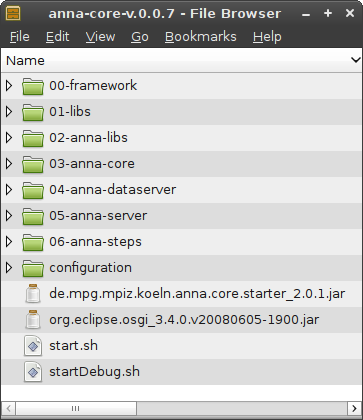
\includegraphics[scale=0.7]{pics/coreDir.png}
	\caption[coreDir]{
	\textbf{coreDir.}
	something.}
	\end{center}
	\label{fig:programOrganisationOverview3ScaledWithAlpha}
\end{figure}

Das Programm wird über eine batch-Datei gestartet,
die wiederum das OSGi Framework startet:
\begin{verbatim}
start.sh:
java -Xmx1024m -jar org.eclipse.osgi_3.4.0.v20080605-1900.jar
-clean\end{verbatim}
Das OSGi Framework ist so konfiguriert (\code{configuration/config.ini}), dass
es beim Starten automatisch das Bundle
\begin{verbatim}
de.mpg.mpiz.koeln.anna.core.starter_2.0.1.jar
\end{verbatim}
installiert und startet.
Dieses Bundle initialisiert und startet nun die Pipeline, indem es alle Bundles,
die sich in den Verzeichnissen \code{00-} bis \code{06-} befinden, startet
\todo{startet startet startet}. Im Verzeichnis \code{06-} sollten sich dabei
alle Step-Bundles befinden, die in der Pipeline genutzt werden sollen.



\section{Server}
Der Server der Pipeline besteht aus zwei Elementen: Zum einen ein
\code{StepExecutor}, der die einzelnen Steps zur Ausführung bringt, sowie der
\code{DataProxy}, der den Zugriff auf das \code{DataBean} Objekt
\todo{schon erklärt?} steuert. \code{StepExecutor} sowie \code{DataProxy} sind
als OSGi Service implementiert. Den einzelnen Clients ist es somit möglich, über OSGi
spezifische Möglichkeiten \todo{hmmm} eine Server Refrenz abzufragen und sich
dort entsprechend anzumelden.
\index{Server|see{Pipeline-Server}}
\index{Pipeline-Server}
\index{Data Proxy}
\index{OSGi Service}
\index{DataBean}
%\lstinputlisting[frame=single,label=server,caption=Application
%Server]{code/server}

\subsection{StepExecutor}
Wird ein Step am Server registriert, wird er an einen StepExecutor übergeben,
der die Ausführung des Steps überwacht und steuert. Er ruft im wesentlichen
die drei Callback Methoden von \code{Step} auf.


\subsection{DataProxy}
Die Pipeline persistiert die (Zwischen-)Ergebnisse einzelner Steps, um bei
einer gewollten oder ungewollten Unterbrechung des Programms die bis dahin
gewonnenen Daten nicht zu verlieren. Eine \code{Step} Implementierung bekommt
beim Aufruf der Callback Methoden eine Refrenz auf einen Data Proxy, über den
die aktuell in der Pipeline verfügbaren Daten abgefragt werden können. Der
Proxy kontrolliert den Zugriff auf die Daten und implementiert dabei alle
Aspekte der Synchronization und Serialisierung der Daten.

\begin{figure}[ht]
	\begin{center}
		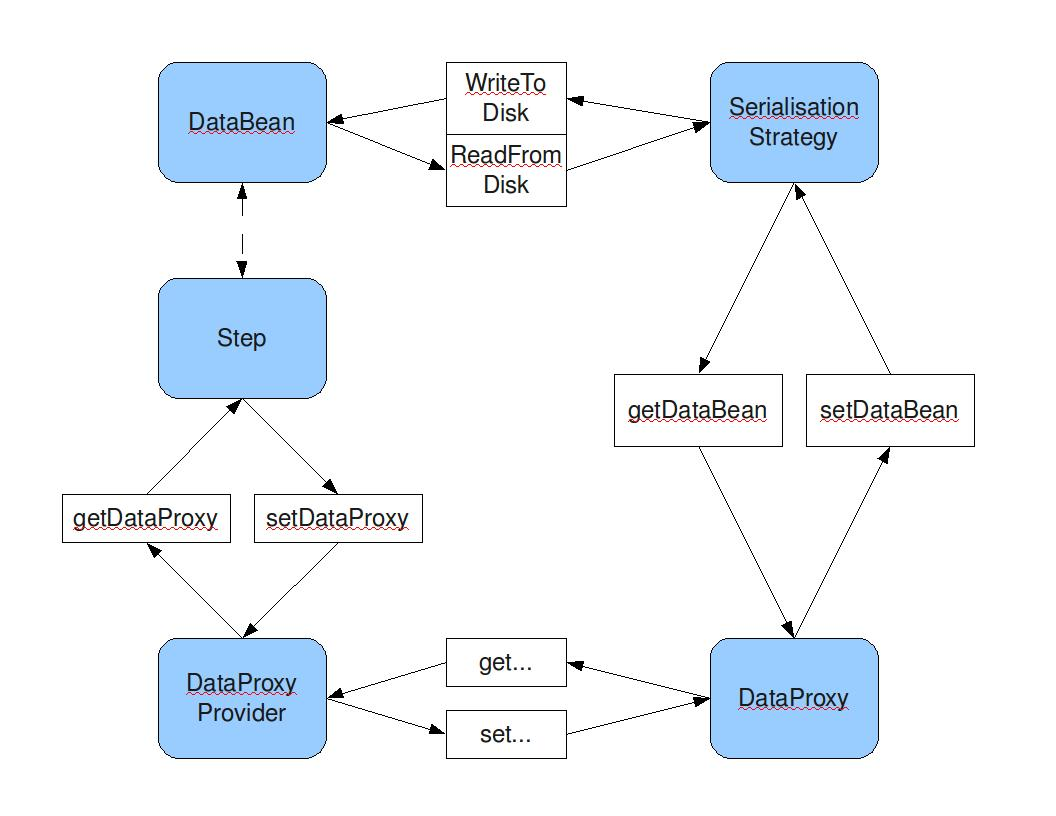
\includegraphics[scale=0.42]{pics/programDataManagment.jpg}
	\caption[Data Management]{
	\textbf{Data Management.}
	something}
	\end{center}
	\label{fig:programDataManagment}
\end{figure}



\index{Pipelineserver}
\index{OSGi Service}




\section{Implementierungen von \code{Step}}
Ein Pipeline Step muss von \code{AbstractStep} erben.
\subsection{Conrad}
Conrad
(\htmladdnormallink{http://www.broadinstitute.org/annotation/conrad/}{http://www.broadinstitute.org/annotation/conrad/})
ist ein \textit{de novo} gene caller, der Genstrukturen wie Exons und Introns
vorhersagen kann.
\index{Conrad} \index{de novo}\index{gene caller}
Die Vorhersage stützt sich dabei auf \textit{semi-Markow Conditional Random
Fields}, kurz \textbf{CRF}.  % wird in hintergründen erwähnt
\index{Markow} \index{Conditional Random Fields} \index{CRF|see{Conditional
Random Fields}}
Conrad benötigt für seine Genvorhersage eine FASTA-Datei mit einer oder
mehreren zu analysierenden DNA-Sequenzen, sowie eine Binärdatei, die Parameter
für den CRF-Alorithmus entält.
Diese Binärdatei wird in einem Trainingslauf erstellt, der vor der
eigentlichen Genvorhersage durchgeführt wird. Hierbei wird der CRF-Algorithmus
auf die Eingabesequenz trainiert, um die Qualität der Genvorhersage
zu maximieren. Dieser Trainingslauf benötigt eine FASTA-Datei mit
DNA-Sequenzen, die Gene enthalten, sowie eine GFF-Datei mit Annotationen zu
diesen Genen.
Die DNA-Sequenzen, die für das Training herangezogen werden, bestimmen direkt
die Qualität der späteren Genvorhersage:
Je \enquote{ähnlicher} die Trainingssequenzen den Sequenzen für die
Vorhersage sind, desto genauer wird das Ergebnis.
\citep{doherty_gene_2007}

Um einen Eindruck von der Qualität der Genvorhersage zu gewinnen, wurden
mehrere Trainings- und Vorhersage-Schritte mit einem Beispieldatensatz aus dem
Conrad-Packet durchgeführt, deren Ergebnisse dann kreuzvalidiert wurden.
Der Beispieldatensatz beinhaltete 574 Sequenzen von \texttt{Aspergillus niger},
die dazu im Verhältnis 1:10 in zwei Datensätze \enquote{testing} und
\enquote{training} aufgeteilt wurden. Das Training erfolgte mit dem
\enquote{training}-Datensatz, die anschliessende Vorhersage wurde für beide
Datensätze durchgeführt.
\index{Aspergillus niger}

Das Ergebnis hieraus war also zum einen eine Vorhersage für eben die Sequenzen,
mit denen Conrad zuvor trainiert wurde, zum Anderen eine Vorhersage für unbekannte
Sequenzen, welcher allerdings ein optimales Training vorrausgegangen war.

Das Ergebnis der Genvorhersage für die beiden Datensätze \enquote{training} und
\enquote{testing} stellt sich wie folgt dar:\\
Die Werte für den \enquote{training}-Datensatz sind generell relativ konstant,
für den \enquote{testing}-Datensatz sind sie weiter gestreut.
Diese Verteilung ist zu erwarten und zeigt ein ausgewogenes Training.
Das bei einem Training oft auftretende \textit{over fitting} ist nicht
festzustellen.
\index{over fitting}
Die Qualität der Genvorhersagen stellt sich in sechs Kategorien dar:
\begin{description}
\item[prediction sensitivity for coding exons] ist das Verhältnis
der gefundenen Exons zu den tatsächlichen vorhandenen Exons.
\item[prediction specificity for coding exons] \ldots
\item[prediction sensitivity for coding nucleotides] \ldots
\item[prediction specificity for coding nucleotides] \ldots
\item[perfectly predicted sequences] ist das Verhältnis aller
vollständig korrekt vorhergesagten Exons zu der Gesamtmenge an Exons.
\item[nucleotide hidden state agreement] ist das Verhältnis der vorhergesagten
Basen-\enquote{Zustände} zu den tatsächlichen Basen-Zuständen.
\end{description}

\begin{figure}[ht]
	\begin{center}
		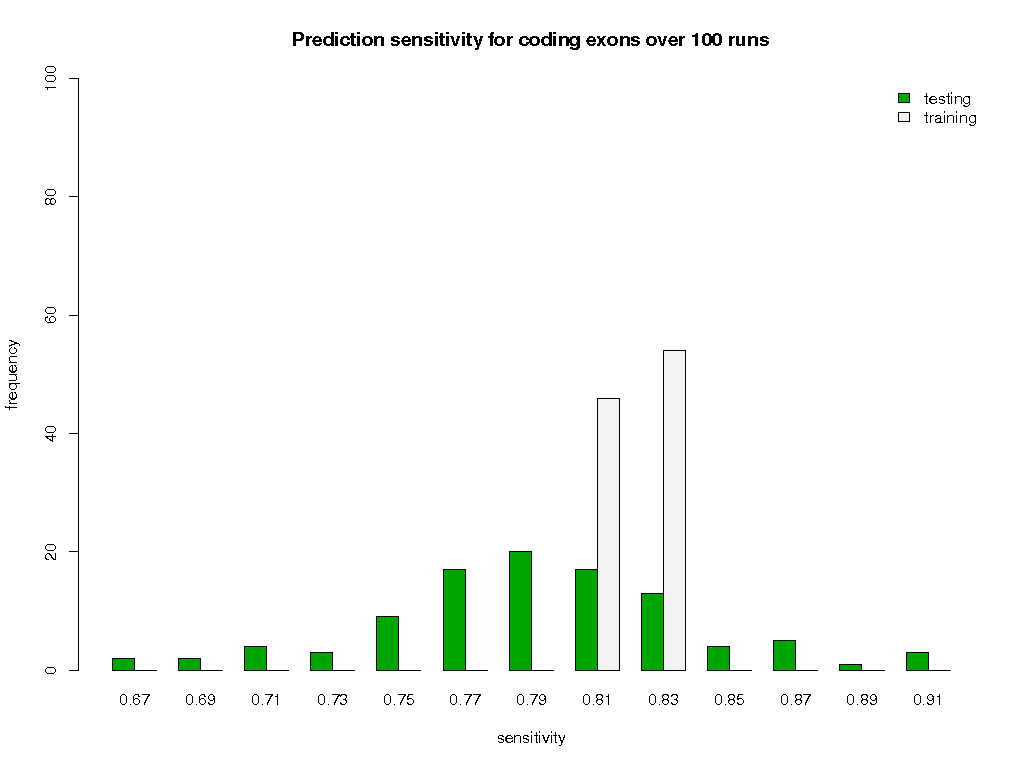
\includegraphics[scale=0.42]{pics/codingExons_sens.png}
	\caption[Prediction sensitivity for coding exons over 100 runs]{
	\textbf{Prediction sensitivity for coding exons over 100 runs.}
	something}
	\end{center}
	\label{fig:codingExons_sens}
\end{figure}

\begin{figure}[ht]
	\begin{center}
		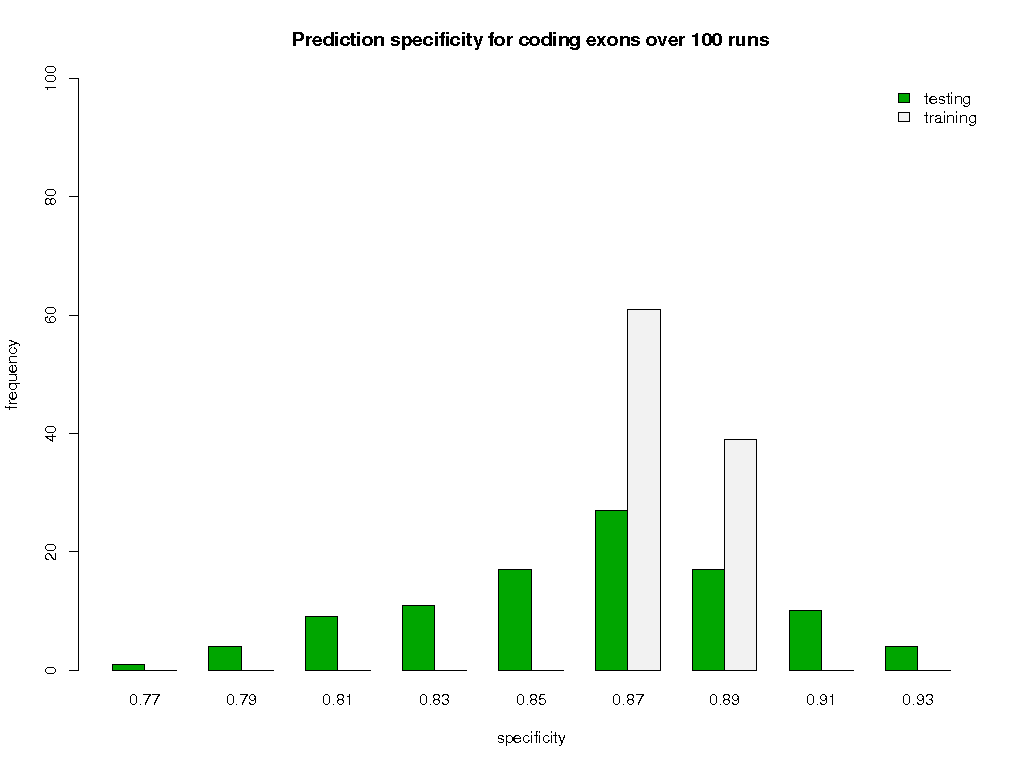
\includegraphics[scale=0.42]{pics/codingExons_spec.png}
	\caption[Prediction specificity for coding exons over 100 runs]{
	\textbf{Prediction specificity for coding exons over 100 runs.}
	something}
	\end{center}
	\label{fig:codingExons_spec}
\end{figure}

\begin{figure}[ht]
	\begin{center}
		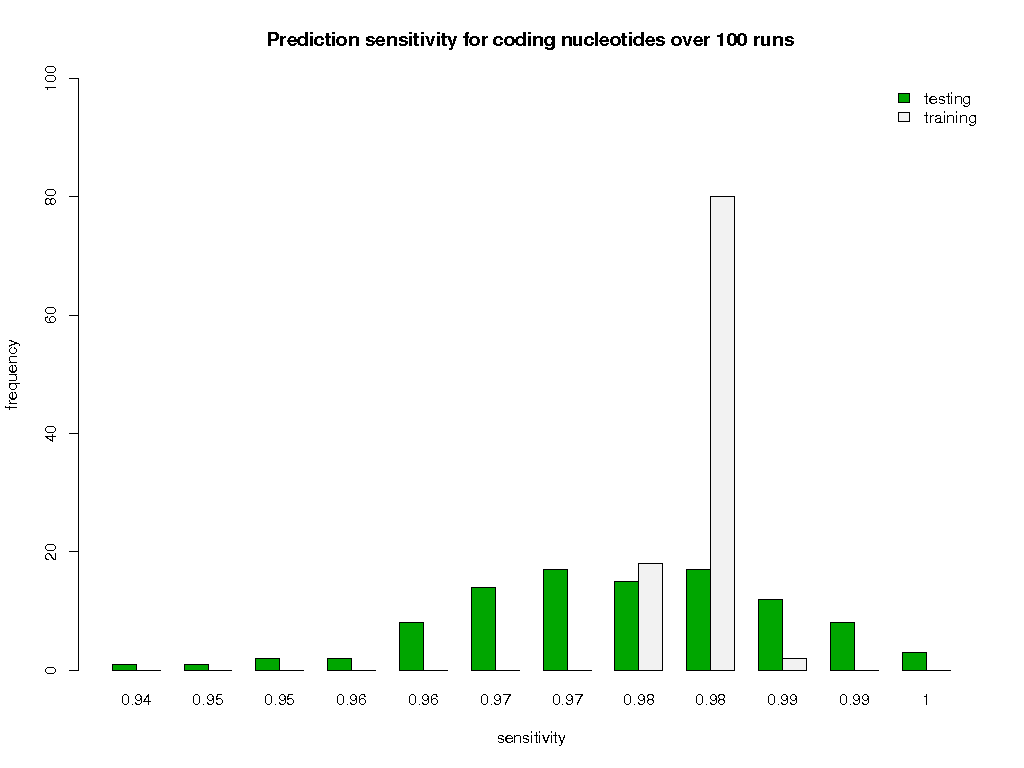
\includegraphics[scale=0.42]{pics/codingNucleotides_sens.png}
	\caption[Prediction sensitivity for coding nucleotides over 100 runs]{
	\textbf{Prediction sensitivity for coding nucleotides over 100 runs.}
	something}
	\end{center}
	\label{fig:codingNucleotides_sens}
\end{figure}

\begin{figure}[ht]
	\begin{center}
		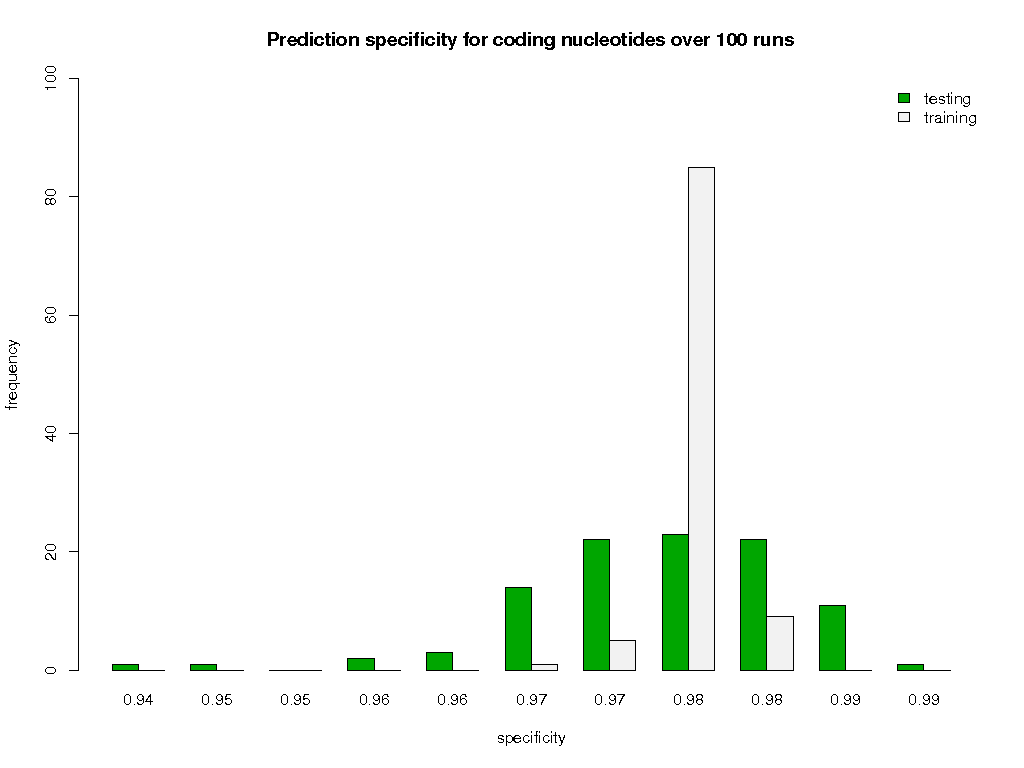
\includegraphics[scale=0.42]{pics/codingNucleotides_spec.png}
	\caption[Prediction specificity for coding nucleotides over 100 runs]{
	\textbf{Prediction specificity for coding nucleotides over 100 runs.}
	something}
	\end{center}
	\label{fig:codingNucleotides_spec}
\end{figure}

\begin{figure}[ht]
	\begin{center}
		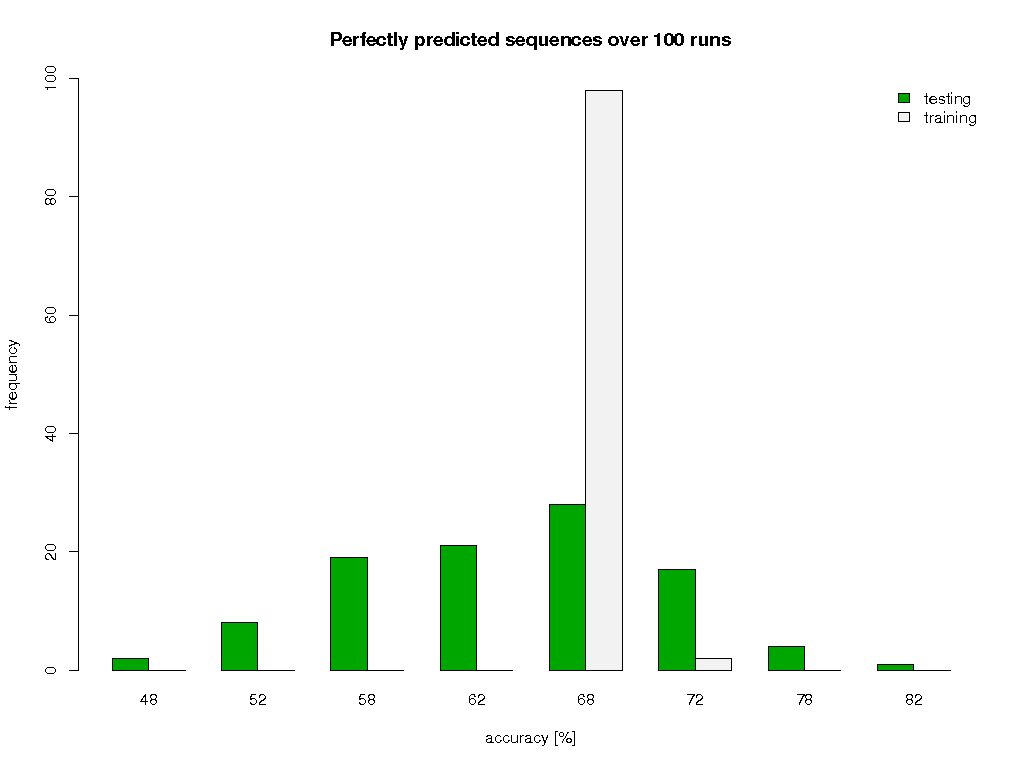
\includegraphics[scale=0.42]{pics/perfect2.png}
	\caption[Perfectly predicted sequences over 100 runs]{
	\textbf{Perfectly predicted sequences over 100 runs.}
	something}
	\end{center}
	\label{fig:perfect2}
\end{figure}

\begin{figure}[ht]
	\begin{center}
		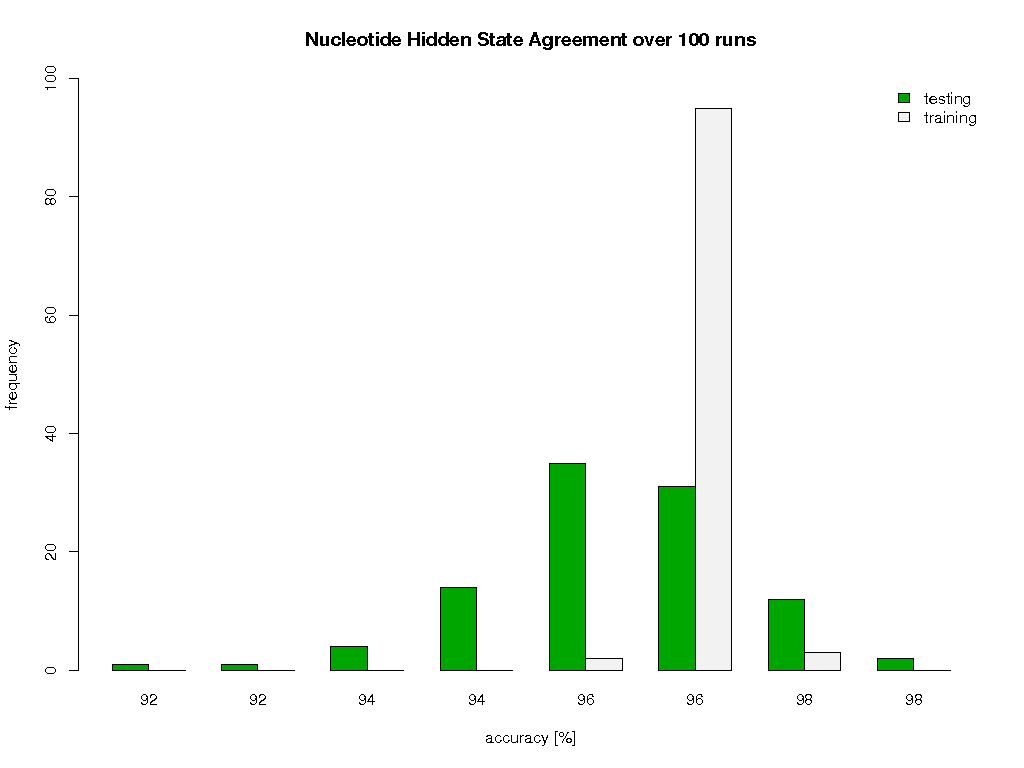
\includegraphics[scale=0.42]{pics/agree2.png}
	\caption[Nucleotide Hidden State Agreement over 100 runs]{
	\textbf{Nucleotide Hidden State Agreement over 100 runs.}
	something}
	\end{center}
	\label{fig:agree2}
\end{figure}

\paragraph{Conrad-local}
\paragraph{Conrad-lsf}
\subsection{RepeatMasker}
RepeatMasker
(\htmladdnormallink{http://www.repeatmasker.org/}{http://www.repeatmasker.org/})
ist ein Open Source Projekt, das repetetive Elemente einer Sequenz
\enquote{maskiert}, um so Rauschen während ähnlichkeitsbasierter Suchen zu
unterdrücken.
Die Maskierung kann entweder durch das Ersetzten der betroffenen Sequenzen
durch \enquote{N}'s bzw. \enquote{X}'s oder auch durch Ändern der Basen zur
Kleinschreibweise erfolgen.
Letzteres wird beispielsweise von \textit{BLAST} erkannt, was zur Folge hat,
dass diese Sequenzabschnitte nicht in der Suche berücksichtigt werden.
Die ursprüngliche Sequenzinformation bleibt auf diese Weise	erhalten.

\paragraph{RepeatMasker-local}

\paragraph{RepeatMasker-lsf}

\section{Libraries}
Neben den Basisfunktionalitäten und den bereits erwähnten Steps
beinhaltet Anna noch verschiedene Bundles, die Klassen aus externen Libraries
bereitstellen:
\begin{description}
\item[bioutils] dieses Bundle bringt 
\end{description}
